% !Mode::"XeLaTeX:UTF-8"
\documentclass[UTF8,titlepage]{ctexart}
\usepackage{graphicx}
\usepackage{placeins}
\usepackage{url}
\usepackage{float}
\usepackage{enumerate}
\usepackage{geometry}
\geometry{left=2cm,right=2cm,top=1.5cm,bottom=1.5cm}
\title{GPS模拟器}
\author{孙大伟\hspace{1cm}李承昊\hspace{1cm}王哲宇\\https://github.com/sundw2014/sdr-transmiter}
\date{}
\begin{document}
\maketitle
%\tableofcontents
\newpage
%.\\[7cm]
\section*{背景介绍}
\paragraph*{}GPS由几十颗卫星构成,这些卫星持续不断地发射电磁波。接收机接收电磁波,并从中得到数据,这些数据包含卫星星历、健康状况、电离层修正等,依靠这些信息可以得到卫星的空间坐标。另外,这些GPS信号应用了CDMA技术,这部分信号称为测距码,接收机可以依靠测距码测出信号从卫星到接收机的飞行时间,从而得到一个接收机到卫星的距离,称为伪距。GPS的信号发射在几个频段上同时进行,使用一个频段的数据即可实现定位。最常用的频段是L1频段,这是一个民用频段,其技术细节完全公开,且无任何加密措施。所以L1频段的信号是完全可以伪造的。对GPS信号的攻击可以有两种基本方式,即重放或完全重新生成信号等。
\paragraph*{重放攻击} 重放攻击是最直接的手段,其基本原理就是录制GPS信号后重放。理论上来说录制的采样率最低为GPS基带带宽的两倍,即2MHz左右。但是由于GPS信号功率很低,其数据基本上淹没在噪声中,所以录制的难度会比较大。此方式的优点在于,原理简单,可以攻击有加密的非民用频段。缺点在于,可扩展性差,无法自由修改信号。
\paragraph*{重新生成信号}随着SDR技术的发展,我们完全有可能构造一个发射机,从用户输入的位置数据,直接生成GPS信号,并发射。这种方式的优点在于灵活。
\section*{理论基础}
\subsection*{GPS L1信号的组成}
GPS信号的组成如图\ref{fig:GPSL1}。从图中可知,GPS L1频段信号由载波、PRN码(伪随机噪声码,包括C/A码和P码两部分,由于P码是加密的我们将其忽略,下文PRN码等同于C/A码)、导航报文数据码组成。参考频率$f_0=10.22999999543MHz$。载波频率为$154f_0=1575.42MHz$;PRN码码片速率为$\frac{f_0}{10}=1.023MHz$,长度为1023;导航报文数据码速率为$50Hz$。所以综上可以得到,一个数据码元中包含20460个PRN码元,一个PRN码元包含1540个载波周期。
\begin{figure}[H]
\centering
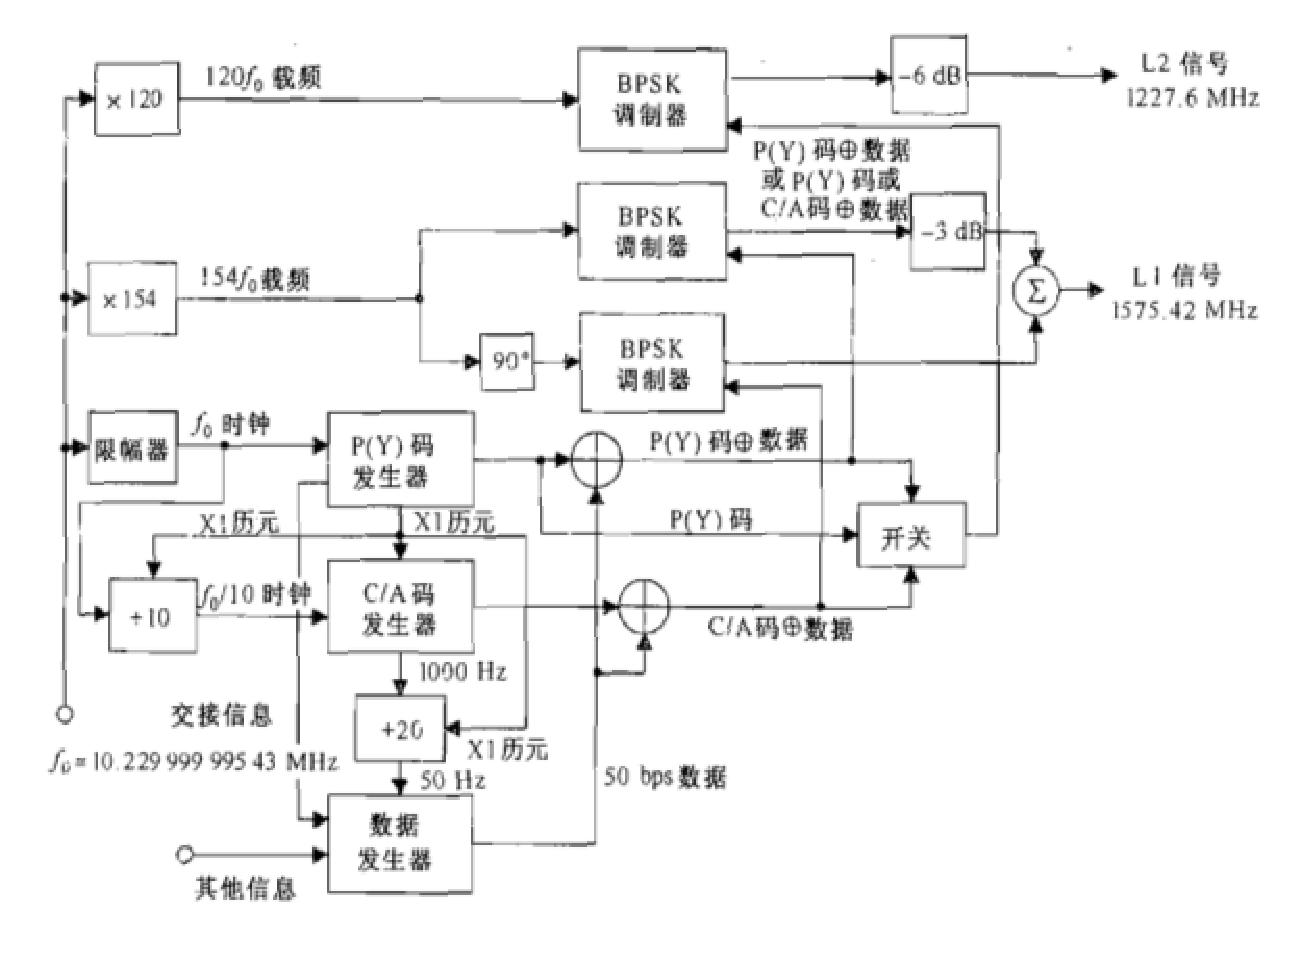
\includegraphics[width = .9\textwidth]{GPSL1.eps}
\caption{GPS L1频段的信号组成}
\label{fig:GPSL1}
\end{figure}
\subsection*{调制方式-二进制相移键控}
二进制相移键控(BPSK)是一种简单的数字信号调节方案,其中在相邻的时间间隔上,取决于所传数字信号是0或1,RF载波分别以其原来的相位或是180度反转的方式传输。BPSK信号可以视为两种时序波形的乘积——未调制的BF载波和数据波,数据波在每个连续的周期($\frac{1}{R_b}$)内取值为+1或-1,其中${R_b}$是以bps来表示的数据率。在很多系统中采用前向纠错,根据一些预定的方法在信道上传输冗余的比特,使得接收机能够检测和纠正可能产生的误差、干扰或衰落造成的错误。
\subsection*{CDMA基础-直接序列扩频}
DSSS可以视为BPSK的一种扩展,或是由GPS和其他卫星导航系统所用的其他相移键控调制方法。DSSS信号加上第三个分量称为扩频或PRN波,类似与其他数据波,但符号率要高很多。这种PRN波是完全已知的,至少对于索要服务的接收器而言是如此。用来产生PRN波一个周期的有限比特序列称为一个PRN序列或PRN码。卫星导航使用DSSS波的主要原因有三:首先,也是最重要的,由PRN调制所带来的信号中频繁的相位反转使得接收机能够精密测距。其次,使用来自一个良好设计的集合的不同PRN序列使得接收机能够精密测距。其次,使用来自一个良好设计集合的不同PRN序列使得多颗卫星能够在同一载频上同时传送信号。接收机能够基于不同的码区分这些信号。由于这一点,在一个公用载频上同时传送信号。接收机能够给予不同的码区分多址。
\section*{GPS接收机原理}为了达到欺骗接收机的目的,我们必须对接收机的原理有比较全面的了解。
\subsection*{卫星信号的捕获、跟踪与数据解调}
GPS接收机需要实现的主要功能是复现所捕获卫星的发射的PRN码,并移动这个复现码的相位使之与原码相关。同时GPS必须在载波相位域内监测卫星,其方法是复现载波频率加多普勒。所以,GPS信号的捕获和跟踪过程是二维的信号复现过程——码和载波这两个维度。在码域内,GPS接收机的目标是使其复现码发生器的瞬时相位与卫星的码相位保持最大相关。 而在处理载波时,接收机要保证在对载波频率的匹配和对卫星频率的跟踪必须同时进行。由此可以知道,要实现欺骗的目的,必须根据星历复现接收机相对于卫星产生的多普勒相移。GPS接收机包括了二维稳态跟踪过程、二维的搜索和捕获等过程,我们在其中选择了一些与本课程相关的内容进行了学习与总结。
\subsubsection*{环路滤波器}
\paragraph*{}环路滤波器的作用是降低噪声以便在其输出端对原始信号产生精确的估计,环路滤波器的结束和噪声带宽也决定了环路滤波器对信号的动态响应。通过信号与系统课程中学到的滤波器设计和系统框图绘制的知识,我们可以看到,环路滤波器的输出信号实际上要与原始信号相减以产生误差信号,误差信号再反馈回滤波器输入端形成闭环过程。
\paragraph*{}图\ref{fig:conCircle}和图\ref{fig:disCircle}所示的分别为1,2,3阶模拟、数字滤波器的框图表示。实际运用中,可以根据公式确定框图中各参数的值,便能完成GPS接收机中的降噪滤波。
\begin{figure}[H]
  \begin{tabular}{cc}
    \begin{minipage}{.5\textwidth}
    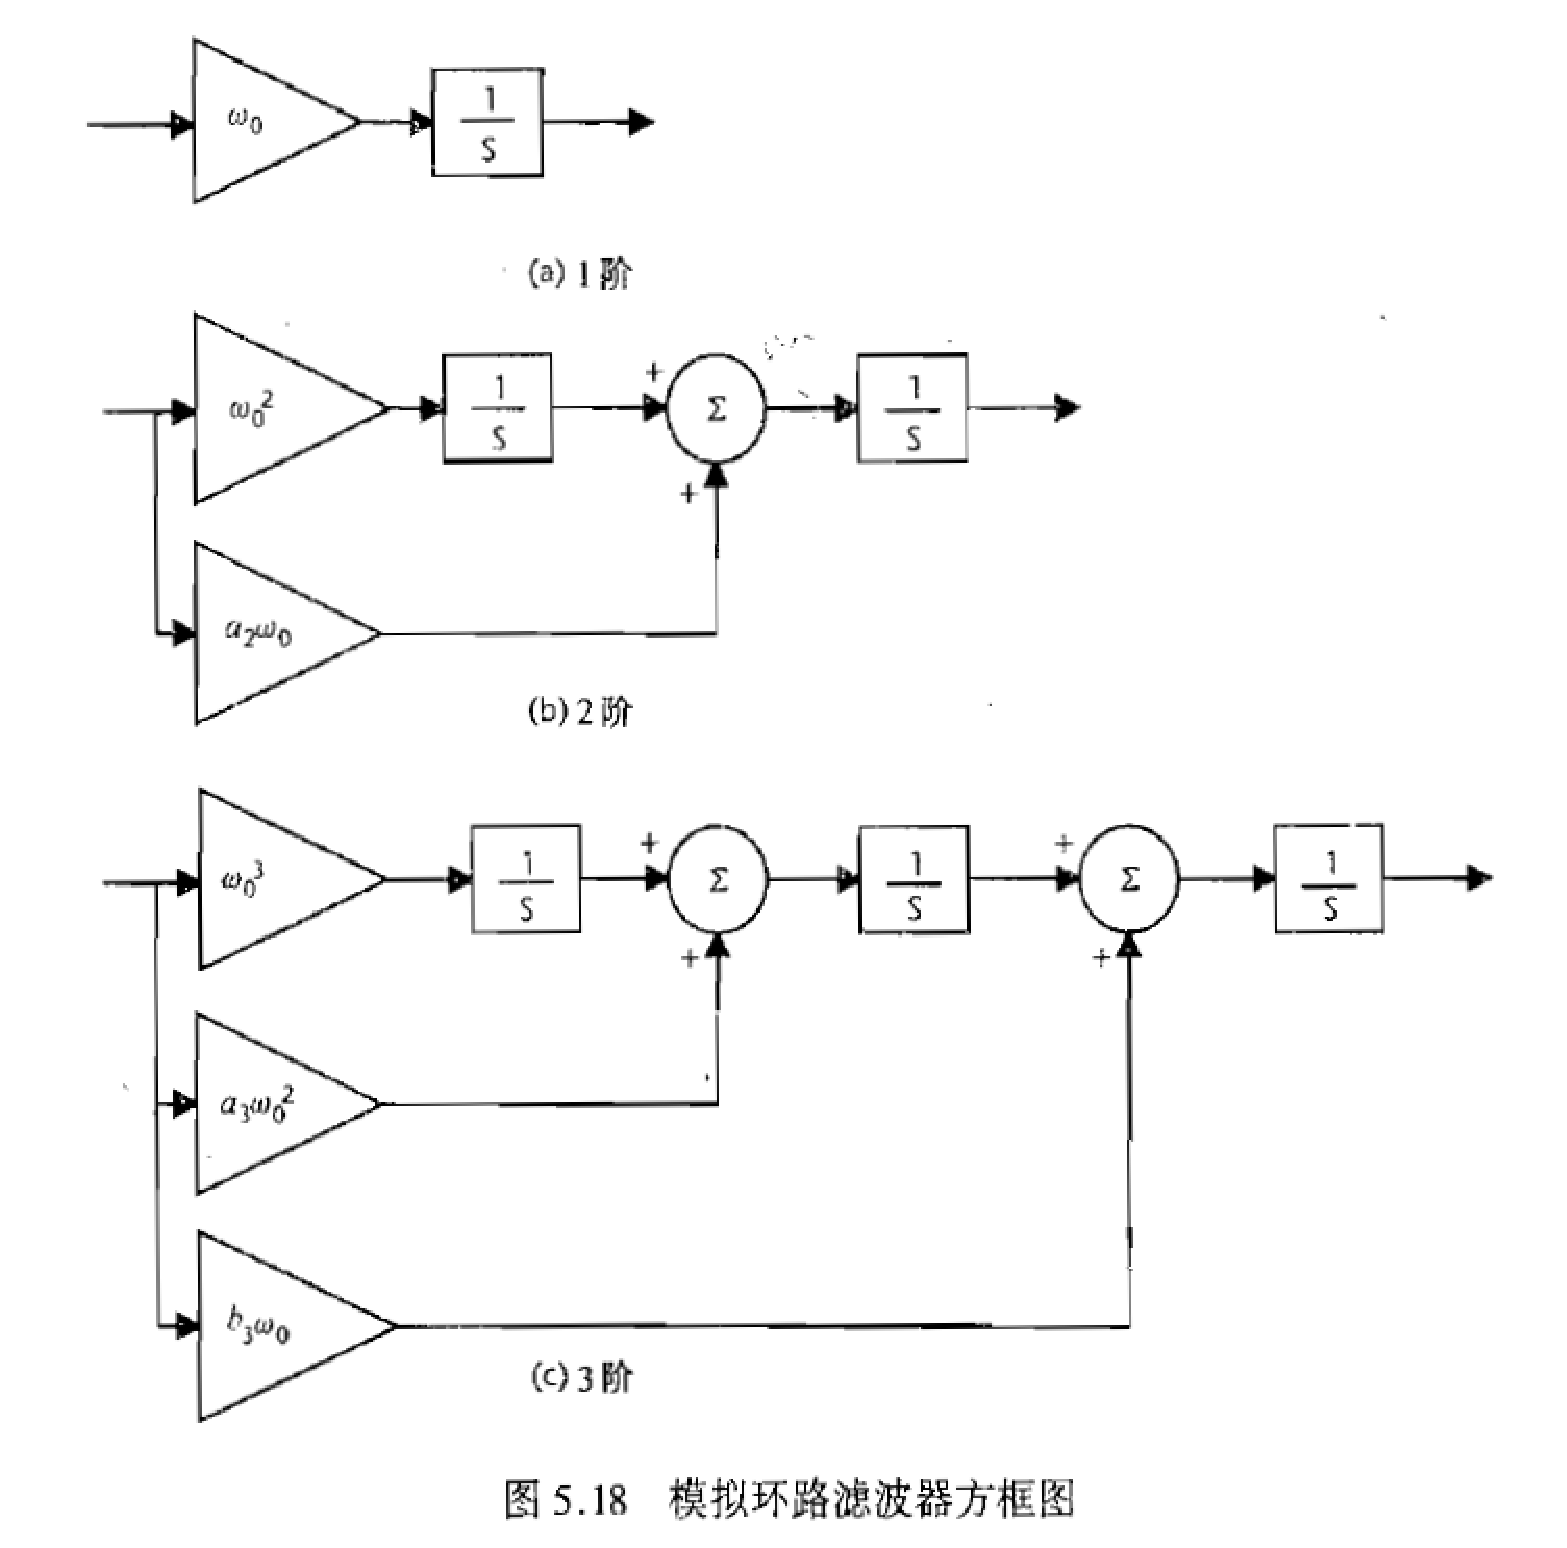
\includegraphics[width = \textwidth]{conCircle.eps}
    \caption{模拟环路滤波器框图\cite{gpsPrin}}
    \label{fig:conCircle}
    \end{minipage}
    \begin{minipage}{.5\textwidth}
    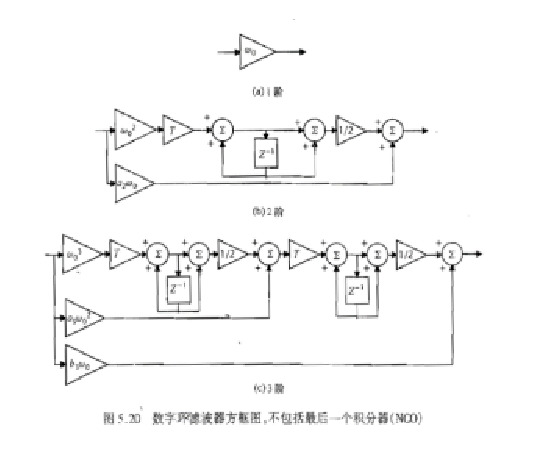
\includegraphics[width = \textwidth]{disCircle.eps}
    \caption{数字环路滤波器框图\cite{gpsPrin}}
    \label{fig:disCircle}
    \end{minipage}
  \end{tabular}
\end{figure}
\subsubsection*{载波跟踪环}
\paragraph*{}载波跟踪环的类型分为锁相环、科斯塔斯锁相环、锁频环。锁相环和科斯塔斯锁相环是最精确的,但对动态应力比锁频环更敏感。GPS接收机的设计中在设计载波跟踪环的预检测积分时间、鉴别器和环路滤波器功能要解决一个矛盾:为了容忍动态应力,预检测积分时间应当短,鉴别器应为一个锁频环,载波环滤波器的带宽应该宽;同时,为了使载波量测量精确,预检测积分时间应该长,鉴别器应为锁相环。所以为了解决这个矛盾,必须做出一些折中—— 一个良好设计的GPS接收机应该采用短的预检测积分时间,用锁频环和宽带的载波环滤波器把它的载波跟踪环闭合起来。
\subsubsection*{GPS接收机的结构}
\paragraph*{}大多数现代的GPS接收机方案是数字接收机。这种接收机方案已迅速趋向于越来越高级的数字期间组合的方向。另外,微处理器及其特殊的同类——DSP的功能日益强大,性价比日益升高,使得人们不需要使用定制的数字器件即可开发出软件定义的接收机。如gnss-sdr项目\cite{gnssSdr}就是一个基于SDR设备的软件gnss接收机。因此,我们用现代数字GPS接收机的高层方框图代表一般GPS接收机的结构,如图\ref{fig:digArch}所示。
\paragraph*{}所有卫星的射频信号由具有接近于半球形增益覆盖的右旋圆极化天线接收,这些射频信号经低噪声前置放大器放大,这个前放实际上确定了接收机的噪声系数。在天线和前放之间可以有一个无源带通前置滤波器,以使带外射频干扰减至最小。然后这些经放大和信号调理的射频信号被来自本地振荡器的混频信号下变到中频,每一级变频器下需要一个本地振荡器。在混频过程之后保留了信号多普勒和PRN码,只是载频降低了,而多普勒仍以原来L波段信号上的多普勒为基准。从模拟到数字的变换过程和自动增益控制功能均在中频上进行。中频必须足够高才能提供足以支撑PRN码码片速率的单边带宽。来自所有视界内GPS卫星的信号均掩埋在中频的热噪声中。
\begin{figure}[H]
\centering
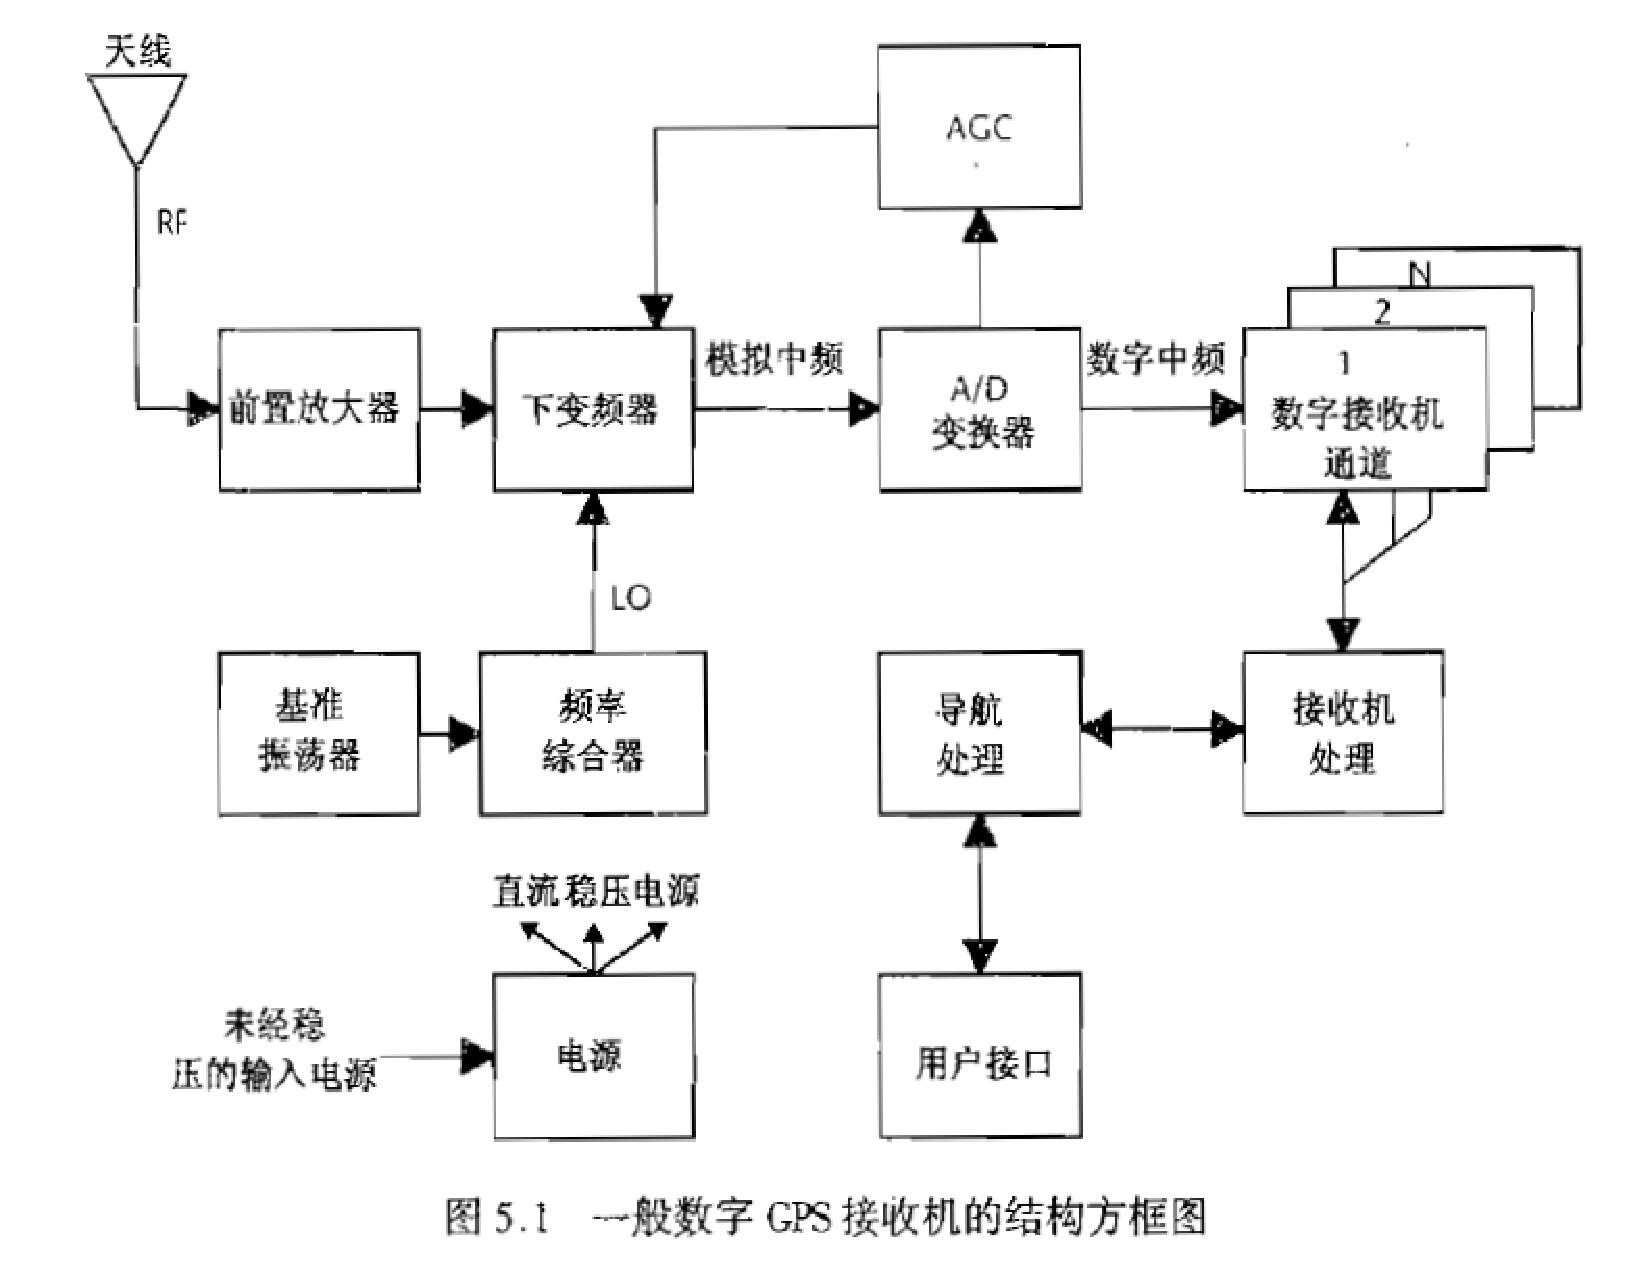
\includegraphics[width = .9\textwidth]{digArch.eps}
\caption{典型数字接收机框图}
\label{fig:digArch}
\end{figure}
\section*{设计与实现}
\subsection*{顶层设计}
从上一节可以知道,我们只要复原出了四颗或四颗以上卫星的信号就能实现GPS欺骗。我们将系统分为软硬件两部分介绍和实现。软件部分包括两部分:上位机程序和单片机程序。上位机程序接受用户输入的坐标文件,里面包含了一个经纬度序列,指定了用户想要模拟的位置或路径,最终生成一个基带信号文件,是基带信号的采样后的序列;单片机程序主要用于接收上位机产生的数字基带信号,并将其应用到DAC上,同时也会配置载波发生器模块的频率。硬件部分由载波发生器模块、混频器、DAC、单片机三部分组成。单片机与上位机通信,同时配置混频器、DAC和载波发生器模块。
\subsection*{软件实现}
\subsubsection*{上位机程序}
上位机程序接受用户输入的坐标文件,里面包含了一个经纬度序列,指定了用户想要模拟的位置或路径。程序每100ms从序列中读取一个点然后将这个点设置为接收机的位置,然后利用星历计算出每个卫星的位置。然后进行一个类似"光线追踪"的操作,得到卫星、地球、接收机的遮挡关系,从而得到接收机视野中可以看到的卫星集合。然后程序进入一个循环,每次循环生成基带序列中的一个采样点,程序在这个循环中维护一个数组$phase[i]$用于记录每个卫星的载波相位。在循环中,计算每个可见卫星的当前PRN值$P[i]$、导航报文数据$D[i]$、速度以及此速度对应的多普勒频偏$f_d[i]$。程序会计算$b[i]=P[i]*D[i]*cos(phase[i])$,并将$\Sigma b[i]$当做基带的一个采样点,写入文件。最后更新每个卫星的载波相位$phase[i]+=f_d[i]*delta$,其中delta为基带信号的采样间隔。可以想像,真正的GPS信号在调制时肯定不会考虑频偏,GPS信号从卫星发出之后,到达接收机时会产生多普勒频偏,相当于原信号在频谱上发生一个偏移$f_d$。接收机会根据星历对这一偏移进行纠正。我们在GPS欺骗过程中,发射机与接收机之间几乎不会有多普勒效应。所以我们在调制时不是直接生成基带信号而是将基带信号与多普勒频率的正弦波相乘得到实际的基带信号,从而可以保证在基带信号调制到载波上时,多普勒频偏也会被调制进去。由于此部分代码过于庞杂,而且我们恰好了解到一个相关的开源项目gps-sdr-sim\cite{gpsSdrSim}。所以我们直接借用了gps-sdr-sim的代码。我们认真阅读了代码,并做了一些测试,可以在版本库的fork版本\cite{gpsSdrSimFork}中查看。
\subsubsection*{单片机程序}
单片机程序主要的工作包括配置载波发生器模块和DAC模块。配置载波发生器模块只是设置其振荡频率为L1载波频率,不在详述。下面介绍DAC模块相关的内容。因为基带采样率为2.6MHz,使用一个8位DAC。所以上位机与单片机之间的传输速率最低位2.6MB/s。所以我们最终决定使用USB进行数据传输。单片机的使用中断将数据输出到DAC的数据端口。
\subsection*{硬件实现}
硬件部分包括单片机、DAC、混频器和载波发生器模块。单片机选用了stm32F407 主频168MHz。DAC选用了AD9708,最大采样率100MS/s。混频器选用的是ADL5801,10MHz至6GHz宽带有源混频器。载波发生器模块使用ADF4351,是一款集成VCO的35MHz至4400MHz频率合成器。载波发生器与混频器之间使用差分接口,保证了低噪声。DAC模块的输出极自带了一个截止频率为100MHz的低通滤波器。
\subsection*{调试过程和成果}
\paragraph*{}我们首先制作一块pcb将USB和DAC模块整合在一起。首先按照预定的方案,使用DMA操作DAC的数据,此时不使用USB,直接将prn码存放在单片机中。
\paragraph*{}实验中发现,单片机不给力,数据更新的速度无法达到要求,实际测试的速率为1MHz左右。我们马上采取了行动,改用了FPGA进行实验。具体思路是将prn码内建在FPGA的ROM中,使用一个时钟信号驱动,数据输出速率轻松达到了100MHz,已经是DAC采样率上限。但是此种方式也有极大的限制,即对FPGA片内资源依赖太严重,预置的码表不能太大。
\subsubsection*{成果} 改用FPGA之后我们做了以下测试。
\paragraph*{}直接将天线接到锁相环模块上查看载波是否已经发射。因为我们的示波器采样率1GS/s,带宽50MHz,测试中观察500MHz的信号就会被示波器衰减到几乎不可测量,为了确认锁相环确实工作在L1频段,我们使用了廉价的SDR设备rtl-sdr搭配一款android app测量了实际频谱,如图\ref{fig:rtlCar}。可见FFT图中确实有明显峰,由于为了省钱没有使用射频功放,所以功率较低。
\paragraph*{}发射19号卫星的prn码,使用手机直接查看gps模块的内部信息。如图\ref{fig:prn19}所示,可以看到19号卫星的信噪比明显的高(测试在室内,理论上如果没有开启欺骗,则不应该跟踪到19号卫星)。
\begin{figure}[H]
  \begin{tabular}{cc}
    \begin{minipage}{.5\textwidth}
    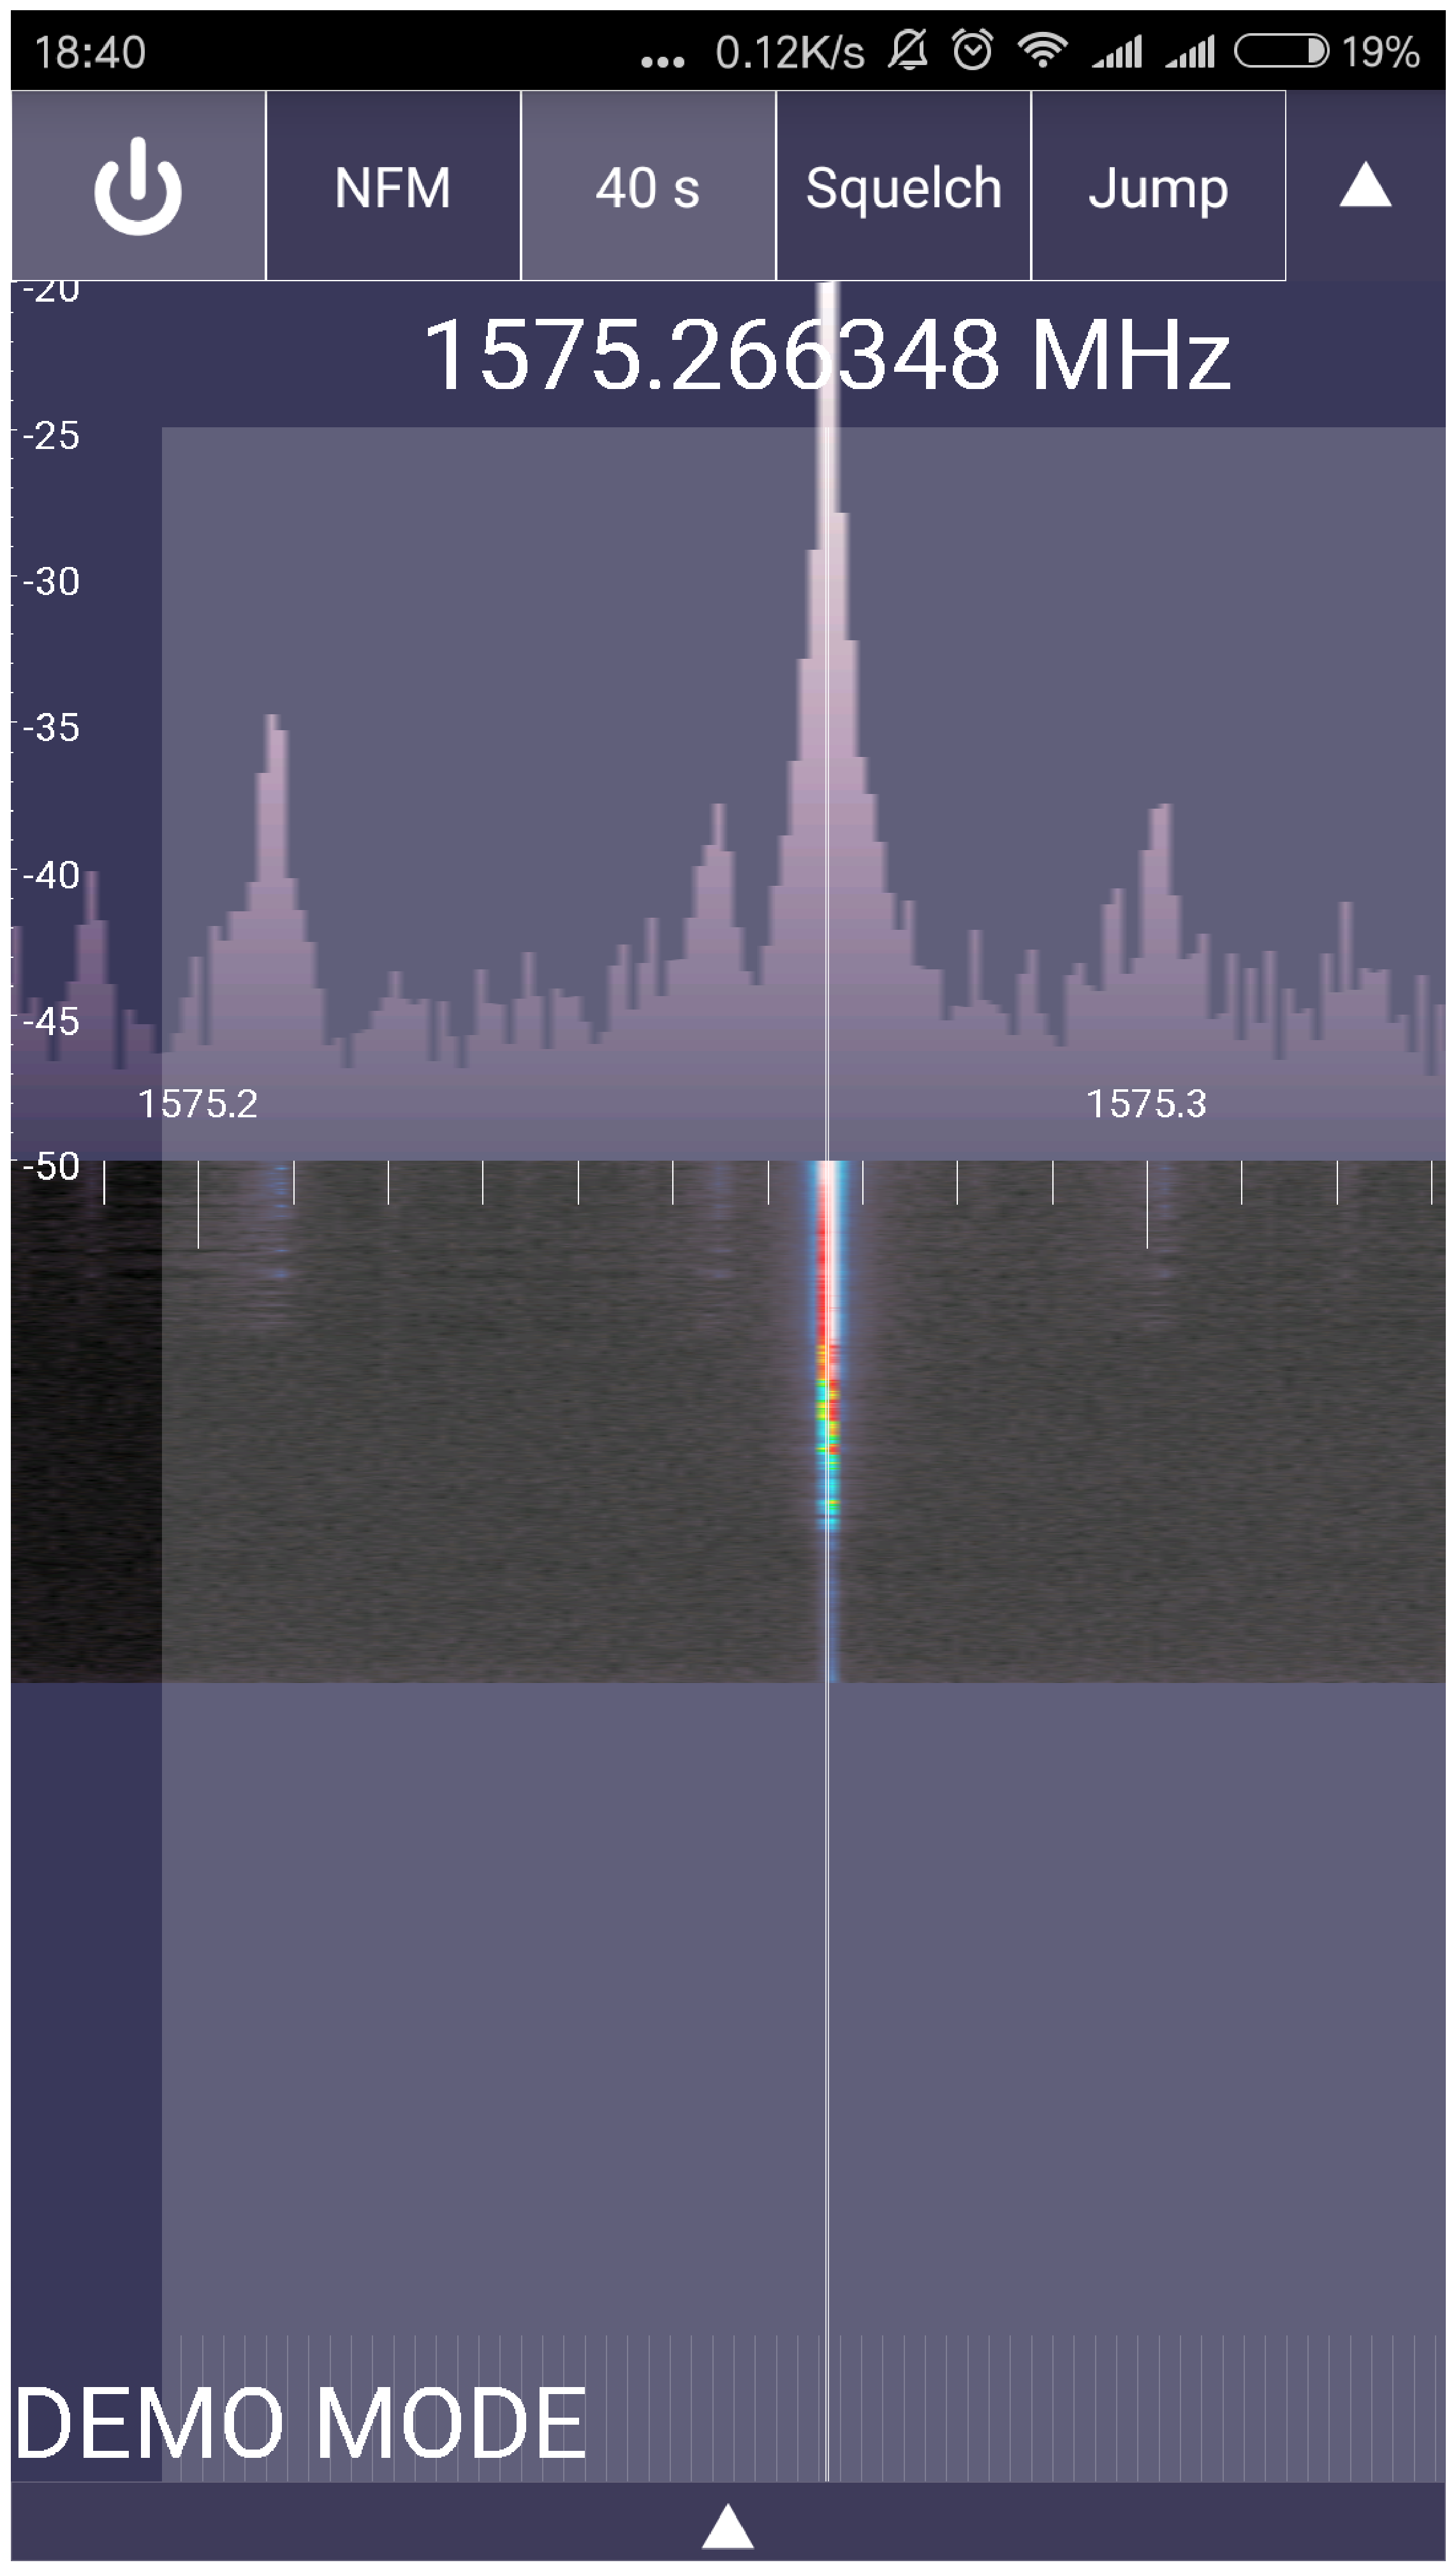
\includegraphics[width = \textwidth]{rtlCar.eps}
    \caption{使用rtl测得的载波频谱}
    \label{fig:rtlCar}
    \end{minipage}
    \begin{minipage}{.5\textwidth}
    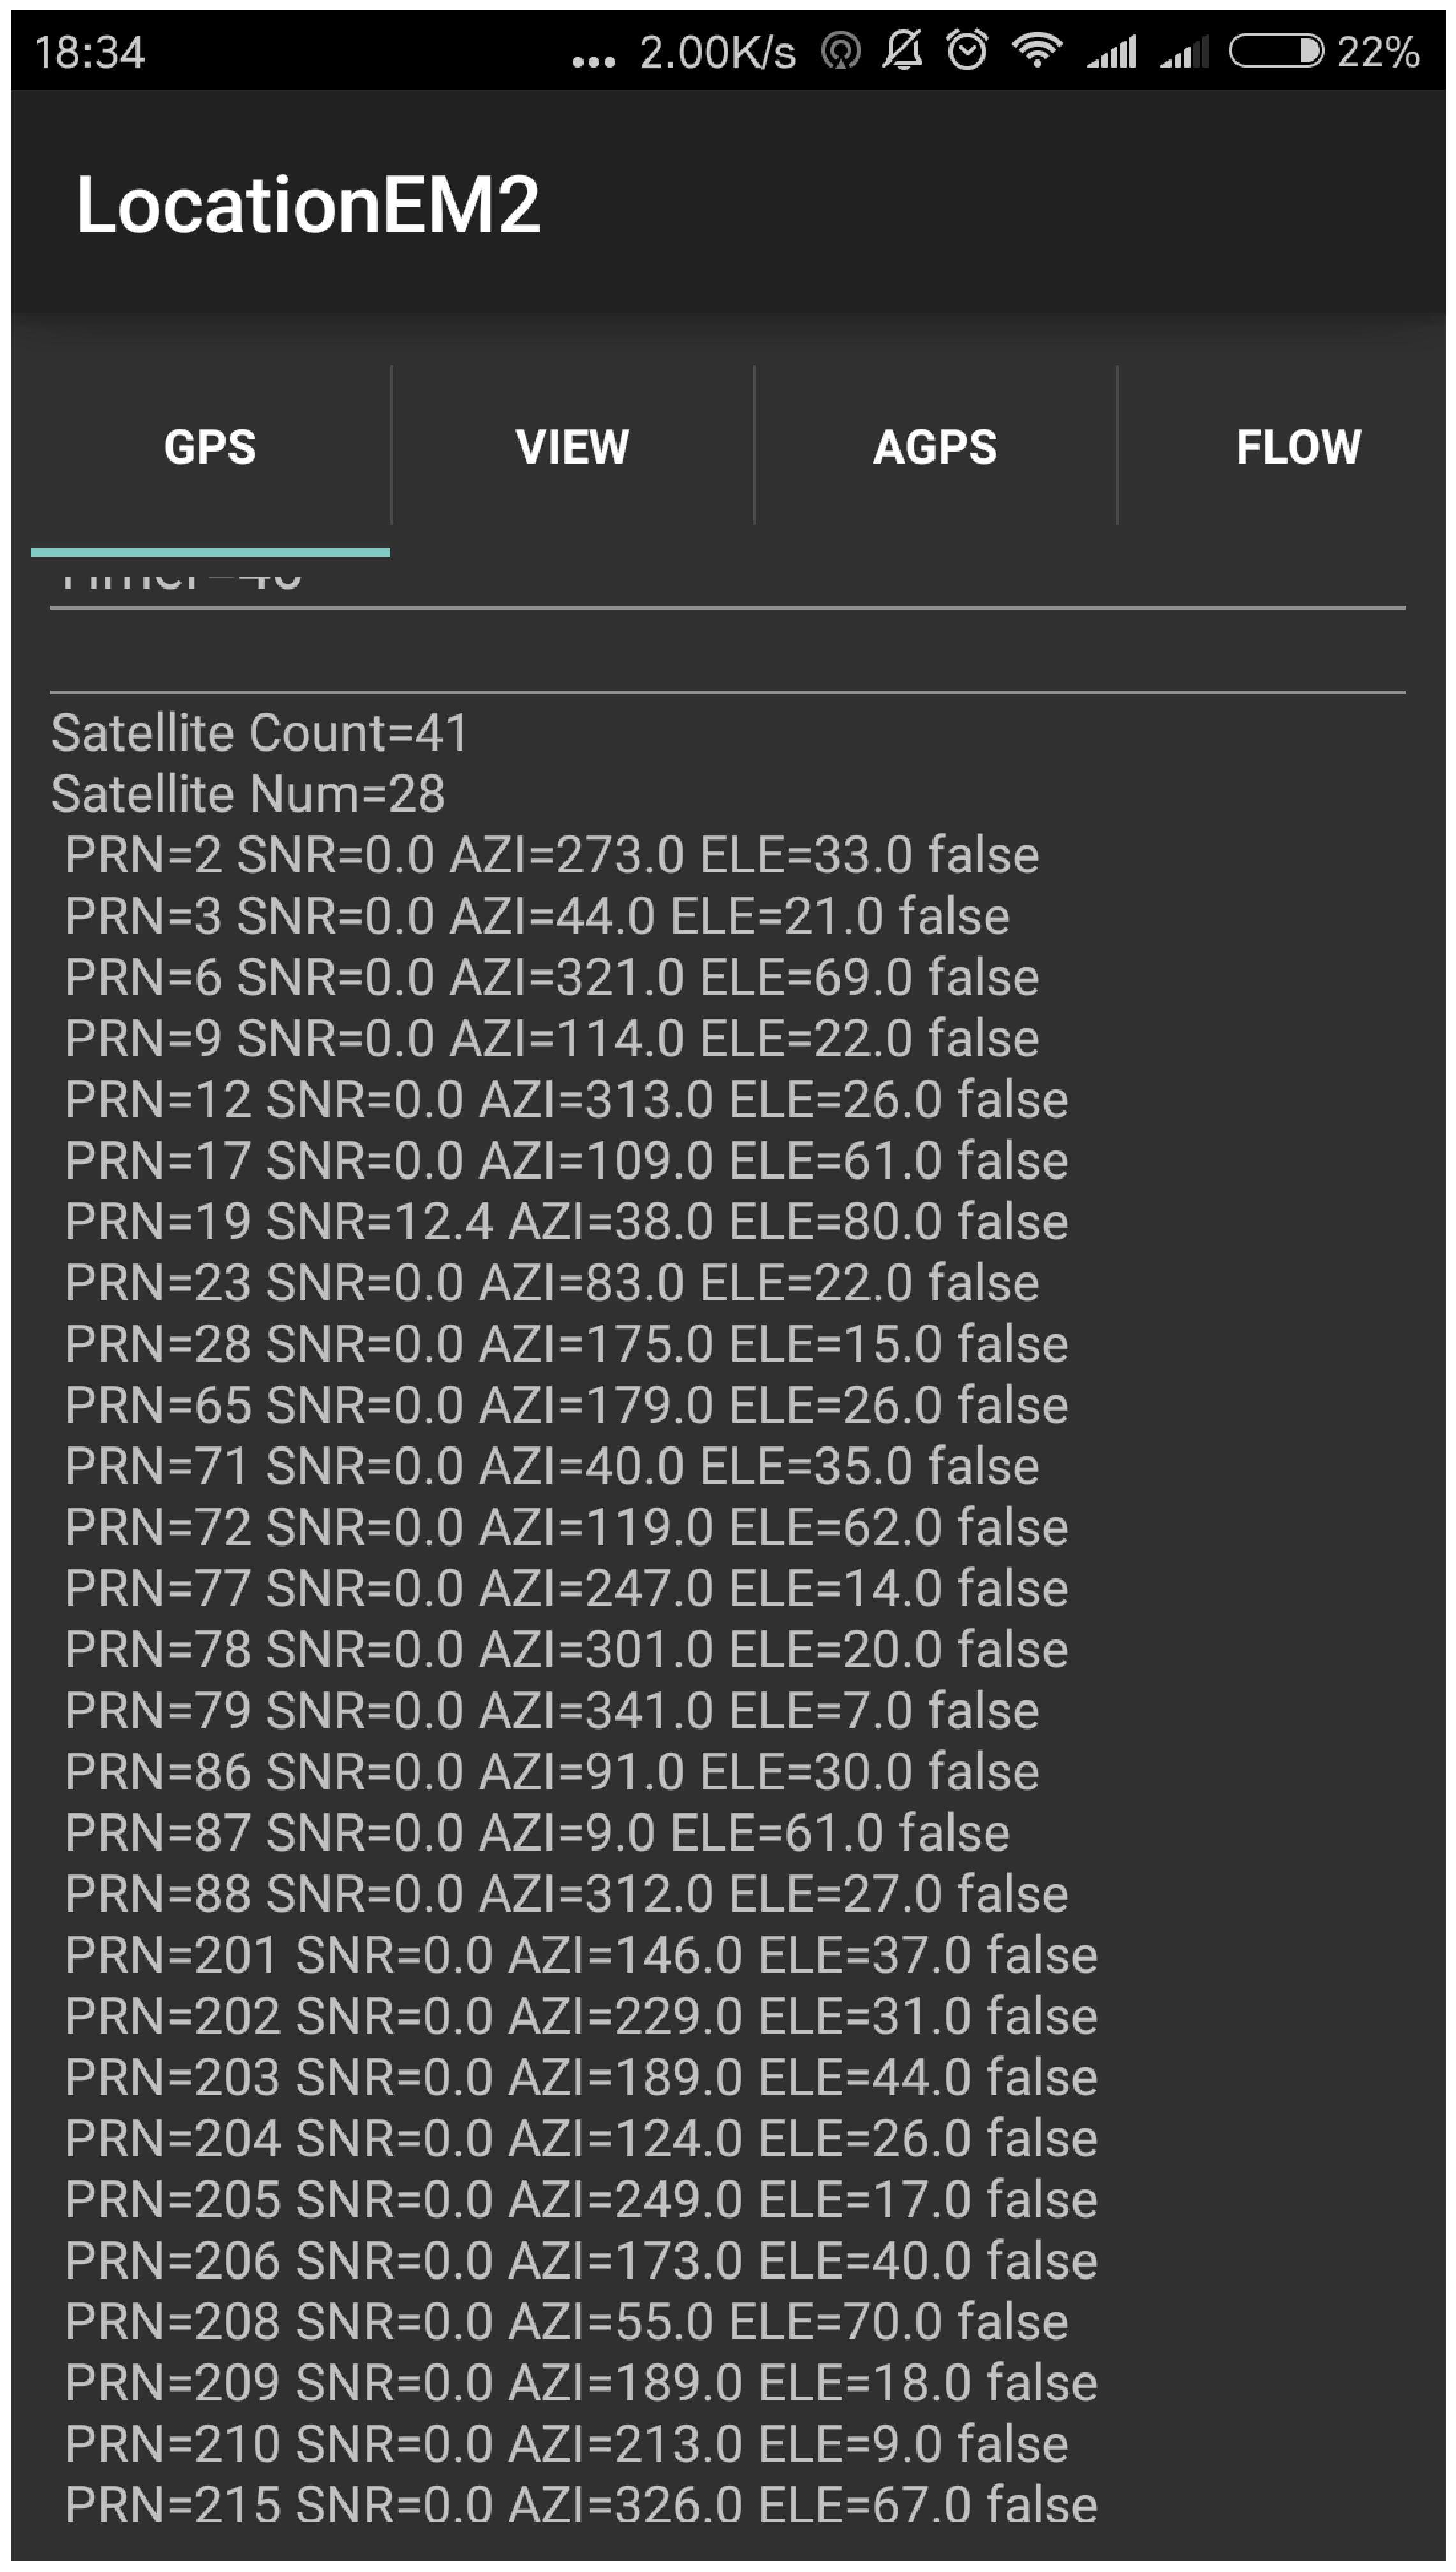
\includegraphics[width = \textwidth]{prn19.eps}
    \caption{手机gps接收机跟踪到的假卫星}
    \label{fig:prn19}
    \end{minipage}
  \end{tabular}
\end{figure}

\begin{figure}[H]
\centering
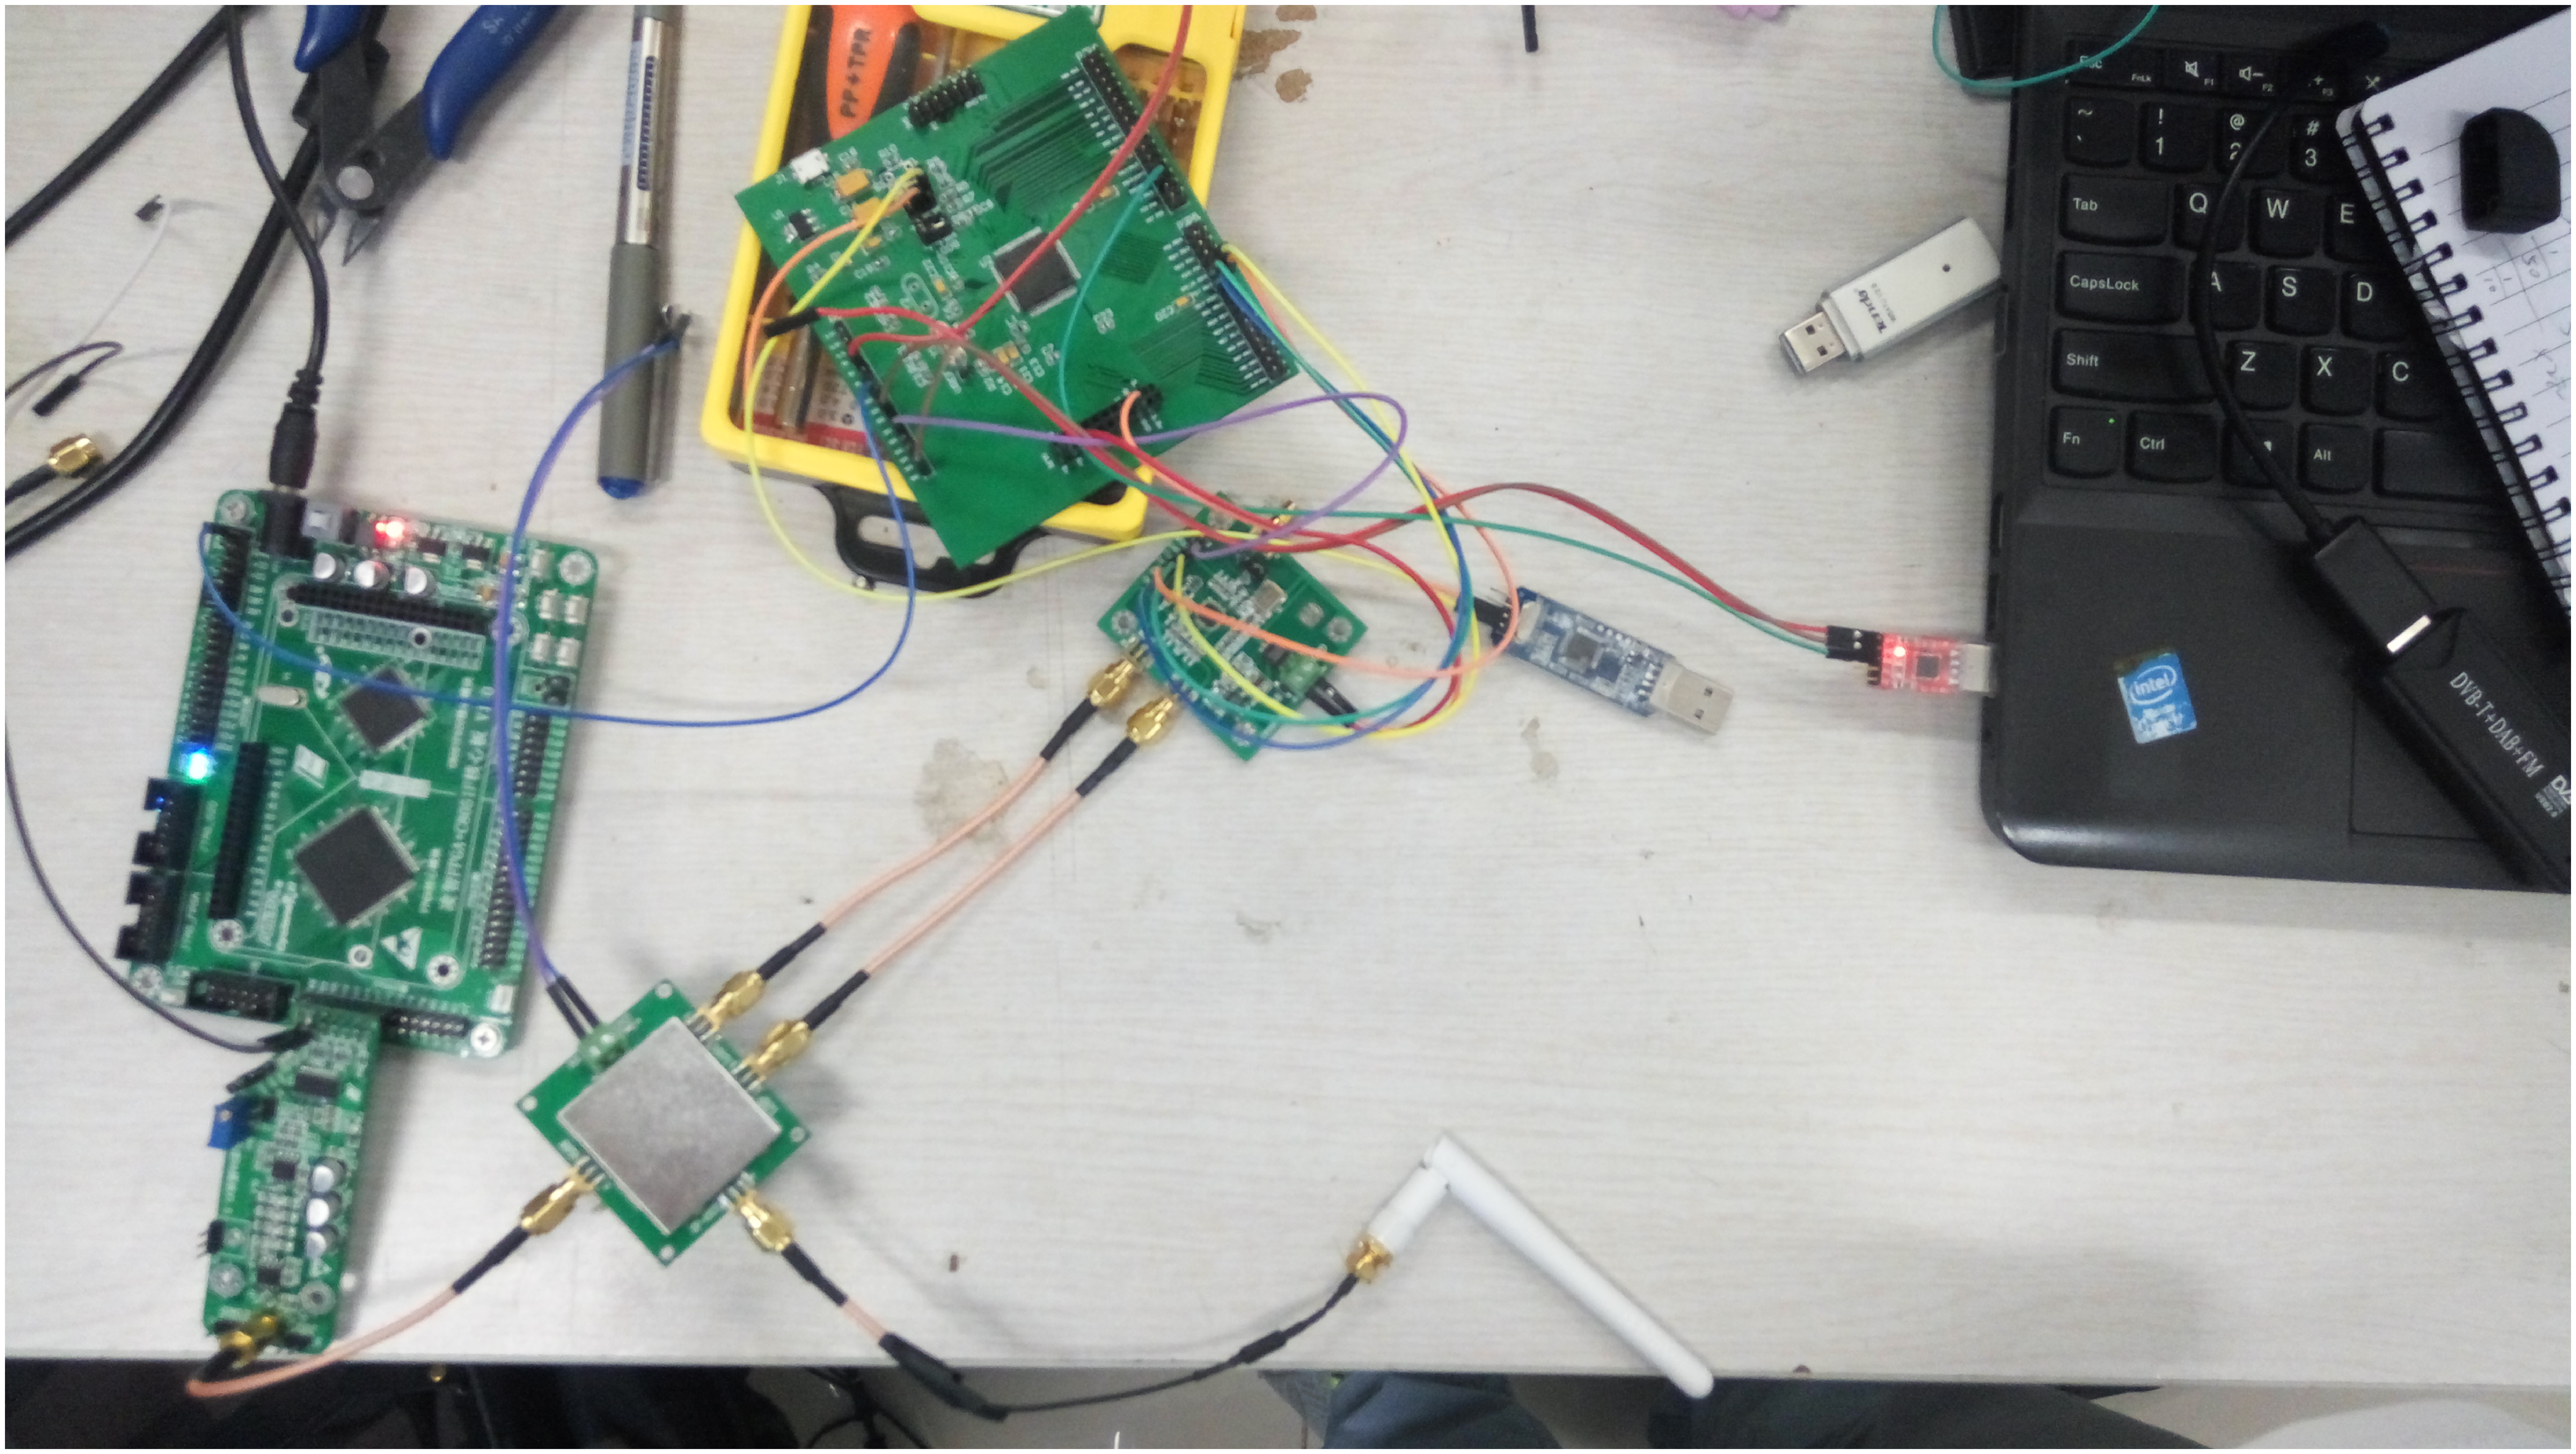
\includegraphics[width = .9\textwidth]{fullStuff.eps}
\caption{硬件整体图}
\label{fig:fullStuff}
\end{figure}

\section*{感想和展望}
我们研究过几款较为成熟的SDR设备的实现。发现在hackRF、bladeRF及USRP三种产品中,hackRF-one使用USB2.0实现与上位机的通信,理论最大速率为480Mbps左右(半双工),bladeRF使用USB3.0理论上限5Gbps,USRP设备产品线庞大,其中B系列使用USB3.0,N系列使用千兆以太网,而SDR设备中最高贵的产品USRP X系列更是使用了光口万兆以太网。而且这些产品中除了hackRF使用CPLD之外,都使用了非常高性能的FPGA,这些FPGA提供了高性能的信号底层处理,如重采样等,同时也为上位机提供了较大的缓冲。这些我们都买不起。所以做了本次实验,想验证一些想法,时间仓促,最终效果不是很满意。
我们将继续维护这个项目。本次实验的所有文件都已上传。项目地址: https://github.com/sundw2014/sdr-transmiter

\newpage
\renewcommand\refname{Reference}
\bibliographystyle{plain}
\bibliography{rep}
\end{document}
